\chapter{Tabulky}

\section{\acs{MIDI} status bajty}
\begin{table}[h]
	\centering
	\caption{Tabulka \acs{MIDI} \texttt{STATUS BAJTŮ} \cite{MIDIspecs}.}
    \begin{tabular}{|l|l|>{\ttfamily}c|>{\ttfamily}c|}
     \hline
     \multicolumn{2}{|c|}{Název} & \textnormal{Hex. hodnota} & \textnormal{Bin. hodnota} \\  
     \hline\hline 
     Note-Off & Nota vypnuta & 0x8n & 1000\,nnnn \\
     Note-On & Nota zapnuta & 0x9n & 1001\,nnnn \\
     Poly Key Pressure & Polyfonický tlakový ovladač & 0xAn & 1010\,nnnn \\
     Control Change & Změna kontroléru & 0xBn & 1011\,nnnn \\
     Program Change & Změna programu & 0xCn & 1100\,nnnn \\
     Channel Pressure & Monofonický tlakový ovladač & 0xDn & 1101\,nnnn \\
     Pitch Bend & Ohyb výšky tónu & 0xEn & 1110\,nnnn \\
     \hline
	\end{tabular}
    \label{tab:MIDIsts}
\end{table}
\newpage

\section{\acs{MoE} značky}\label{chpt:MoEZnacky}
\begin{table}[h]
	\centering
	\caption{Tabulka prvních bajtů \acs{MoE} zpráv.}
	\begin{tabular}{|  >{\ttfamily} c | p{0.7\textwidth} |}
		\hline
		\textnormal{Bajt} & \multicolumn{1}{|c|}{Popis} \\
		\hline \hline
		\vdots & \\
		
		0x08 & Broadcast zpráva od řídícího PC, která sonduje účastníky sítě \\
		
		\vdots & \\

		0x0E & Unicast zpráva od řídícího  PC, která zařízení maže záznam z databáze \texttt{subscriptions}. \\
		
		0x0F & Unicast zpráva od řídícího PC, která zařízení vkládá nový záznam do databáze \texttt{subscriptions}, který je obsahem datagramu \\
		
		\vdots & \\
		
		0x80 & Unicast odpověď na sondáž PC, součástí datagramu je i jeden záznam databáze \texttt{subscriptions} \\

		\vdots & \\

		%0xA2 & Dvoubajtová \acs{MIDI} zpráva pro port A \\
		0xA3 & Tříbajtová \acs{MIDI} zpráva \\
		%0xB2 & Dvoubajtová \acs{MIDI} zpráva pro port B \\
		%0xB3 & Tříbajtová \acs{MIDI} zpráva pro port B \\
		
		\vdots & \\
		
		0xFF & Zpráva \texttt{beacon} sloužící pro upozornění na vlastní přítomnost \\
		\hline
	\end{tabular}
\end{table}


\chapter{Výpisy kódu}
\section{Výpis kódu pro příjem a zpracování \acs{MIDI} zprávy}\label{code:handleMIDI}
\begin{lstlisting}[caption=Výpis kódu pro příjem a zpracování MIDI zprávy]
void handleMIDI()
{
	if (midiSerial.available() == 3)
    {
        _data0 = midiSerial.read();
        _data1 = midiSerial.read();
        _data2 = midiSerial.read();
        sendUDP(_data0, _data1, _data2);
    }
}
	
void sendUDP(byte data0, byte data1, byte data2)
{
	byte srcCh = data0 & 0x0F;
	for (byte i = 0; i < MAX_SUBS; i++)
	{
		if (srcCh == (_subscriptions[i].srcdstChannel 
					       & 0xF0) >> 4)
		{
			data0 = data0 & 0xF0;
			data0 = data0 | (_subscriptions[i].srcdstChannel 
							& 0x0F);
			IPAddress destinationIP = Ethernet.localIP();
			destinationIP[3] = _subscriptions[i].dstIPnib;
			eUDP.beginPacket(destinationIP, MOE_PORT);
			eUDP.write(0xA3);
			eUDP.write(data0);
			eUDP.write(data1);
			eUDP.write(data2);
			eUDP.endPacket();
		}
	}
}
\end{lstlisting}






%\chapter{Některé příkazy balíčku \texttt{thesis}}
%
%\section{Příkazy pro sazbu veličin a jednotek}
%
%\begin{table}[!h]
%  \caption[Přehled příkazů]{Přehled příkazů pro matematické prostředí }
%  \begin{center}
%  	\small
%	  \begin{tabular}{|c|c|c|c|}
%	    \hline
%	    Příkaz    						& Příklad 					& Zdroj příkladu  							& Význam  \\
%	    \hline\hline
%	    \verb|\textind{...}|	& $\beta_\textind{max}$ 	& \verb|$\beta_\textind{max}$|	& textový index \\
%	    \hline
%eličina \\
%	    \hline
%	    \verb|\var{...}| 		& $\var{u}_\textind{in}$ & \verb|$\var{u}_\textind{in}$| & proměnná veličina \\
%	    \hline
%	    \verb|\complex{...}| 	& $\complex{u}_\textind{in}$ & \verb|$\complex{u}_\textind{in}$| & komplexní veličina \\
%	    \hline
%	    \verb|\vect{...}| 		& $\vect{y}$ 						& \verb|$\vect{y}$| & vektor \\
%	    \hline
%	    \verb|\mat{...}| 	& $\mat{Z}$ 						& \verb|$\mat{Z}$| & matice \\
%	    \hline
%	    \verb|\unit{...}| 		& $\unit{kV}$ 						& \verb|$\unit{kV}$|\quad či\ \, \verb|\unit{kV}| & jednotka \\
%	    \hline
%	  \end{tabular}
%  \end{center}
%\end{table}



%%\newpage
%\section{Příkazy pro sazbu symbolů}
%
%\begin{itemize}
%  \item
%    \verb|\E|, \verb|\eul| -- sazba Eulerova čísla: $\eul$,
%  \item
%    \verb|\J|, \verb|\jmag|, \verb|\I|, \verb|\imag| -- sazba imaginární jednotky: $\jmag$, $\imag$,
%  \item
%    \verb|\dif| -- sazba diferenciálu: $\dif$,
%  \item
%    \verb|\sinc| -- sazba funkce: $\sinc$,
%  \item
%    \verb|\mikro| -- sazba symbolu mikro stojatým písmem%
%			\footnote{znak pochází z~balíčku \texttt{textcomp}}: $\mikro$,
%	\item
%		\verb|\uppi| -- sazba symbolu $\uppi$
%			(stojaté řecké pí, na rozdíl od \verb|\pi|, což sází $\pi$).
%\end{itemize}
%%
%Všechny symboly jsou určeny pro matematický mód, vyjma \verb|\mikro|, jenž je\\ použitelný rovněž v~textovém módu.
%%$\upmikro$

%
%\chapter{Druhá příloha}
%
%\begin{figure}[!h]
%  \begin{center}
%    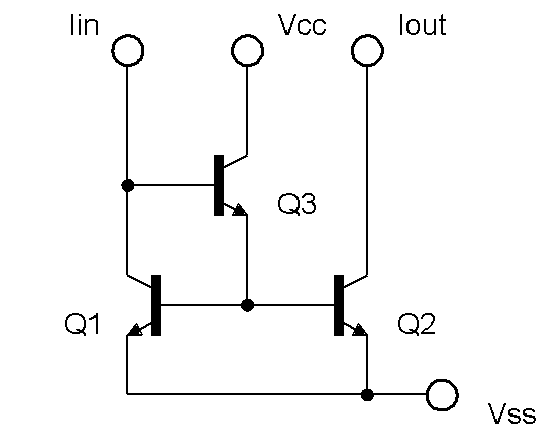
\includegraphics[scale=0.5]{obrazky/ZlepseneWilsonovoZrcadloNPN}
%  \end{center}
%  \caption[Alenčino zrcadlo]{Zlepšené Wilsonovo proudové zrcadlo.}
%\end{figure}
%
%Pro sazbu vektorových obrázků přímo v~\LaTeX{}u je možné doporučit %balíček \href{https://www.ctan.org/pkg/pgf}{\texttt{TikZ}}.
%Příklady sazby je možné najít na \href{http://www.texample.net/tikz/%examples/}{\TeX{}ample}.
%Pro vyzkoušení je možné použít programy QTikz nebo TikzEdt.
%

%
%
%\chapter{Příklad sazby zdrojových kódů}
%
%\section{Balíček \texttt{listings}}
%
%Pro vysázení zdrojových souborů je možné použít balíček \href{https://%www.ctan.org/pkg/listings}{\texttt{listings}}.
%Balíček zavádí nové prostředí \texttt{lstlisting} pro sazbu zdrojových %kódů, jako například:
%%
%\begin{lstlisting}[language={[LaTeX]TeX}]
%\section{Balíček lstlistings}
%Pro vysázení zdrojových souborů je možné použít
%	balíček \href{https://www.ctan.org/pkg/listings}%
%	{\texttt{listings}}.
%Balíček zavádí nové prostředí \texttt{lstlisting} pro
%	sazbu zdrojových kódů.
%\end{lstlisting}
%%
%Podporuje množství programovacích jazyků.
%Kód k~vysázení může být načítán přímo ze zdrojových souborů.
%Umožňuje vkládat čísla řádků nebo vypisovat jen vybrané úseky kódu.
%Např.:
%
%\noindent
%Zkratky jsou sázeny v~prostředí \texttt{acronym}:
%\label{lst:zkratky}
%\lstinputlisting[language={[LaTeX]TeX},nolol,numbers=left, firstnumber=6, %firstline=6,lastline=6]{text/zkratky.tex}
%%
%Šířka textu volitelného parametru \verb|KolikMista| udává šířku prvního %sloupce se zkratkami.
%Proto by měla být zadávána nejdelší zkratka nebo symbol.
%Příklad definice zkratky \acs{symfvz} je na výpisu \ref{lst:symfvz}.
%
%\shorthandoff{-}
%\lstinputlisting[language={[LaTeX]TeX},frame=single,caption={Ukázka sazby %zkratek},label=lst:symfvz,numbers=left,linerange={bsymfvz-\%\%\%\ esymfvz}%,includerangemarker=false]{text/zkratky.tex}
%\shorthandon{-}
%
%\noindent
%Ukončení seznamu je provedeno ukončením prostředí:
%\lstinputlisting[language={[LaTeX]TeX},nolol,numbers=left,firstnumber=26,%linerange=26]{text/zkratky.tex}
%
%\vspace{\fill}
%
%\noindent
%{\bf Poznámka k~výpisům s~použitím volby jazyka \verb|czech| nebo \verb|%slovak|:}\newline
%Pokud Váš zdrojový kód obsahuje znak spojovníku \verb|-|, pak překlad %může skončit chybou.
%Ta je způsobená tím, že znak \verb|-| je v~českém nebo slovenském %nastavení balíčku \verb|babel| tzv.\ aktivním znakem.
%Přepněte znak \verb|-| na neaktivní příkazem \verb|\shorthandoff{-}| %těsně před výpisem a hned za ním jej vraťte na aktivní příkazem \verb|%\shorthandon{-}|.
%Podobně jako to je ukázáno ve zdrojovém kódu šablony.
%
%
%clearpage
%
%\section{Výpis kódu prostředí Matlab}
%a výpisu \ref{lst:priklad.vypis.kodu.Matlab} naleznete příklad kódu pro %atlab, na výpisu \ref{lst:priklad.vypis.kodu.C} zase pro jazyk~C.
%
%lstnewenvironment{matlab}[1][]{%
%iflanguage{czech}{\shorthandoff{-}}{}%
%iflanguage{slovak}{\shorthandoff{-}}{}%
%lstset{language=Matlab,numbers=left,#1}%
%{%
%iflanguage{slovak}{\shorthandon{-}}{}%
%iflanguage{czech}{\shorthandon{-}}{}%
%
%
%begin{matlab}[frame=single,float=htbp,caption={Příklad Schur-Cohnova %estu stability v~prostředí Matlab.},label=lst:priklad.vypis.kodu.Matlab,%umberstyle=\scriptsize, numbersep=7pt]
%% Priklad testovani stability filtru
%
% koeficienty polynomu ve jmenovateli
% = [ 5, 11.2, 5.44, -0.384, -2.3552, -1.2288];
%isp( 'Polynom:'); disp(poly2str( a, 'z'))
%
%isp('Kontrola pomoci korenu polynomu:');
%x = roots( a);
%f( all( abs( zx) < 1))
%   disp('System je stabilni')
%lse
%   disp('System je nestabilni nebo na mezi stability');
%nd
%
%isp(' '); disp('Kontrola pomoci Schur-Cohn:');
%a = zeros( length(a)-1,length(a));
%a(1,:) = a/a(1);
%or( k = 1:length(a)-2)
%   aa = ma(k,1:end-k+1);
%   bb = fliplr( aa);
%   ma(k+1,1:end-k+1) = (aa-aa(end)*bb)/(1-aa(end)^2);
%nd
%
%f( all( abs( diag( ma.'))))
%   disp('System je stabilni')
%lse
%   disp('System je nestabilni nebo na mezi stability');
%nd
%end{matlab}
%
%\noindent
%\begin{minipage}{\linewidth}










%\chapter{Obsah přiloženého CD}
%Nezapomeňte uvést, co čtenář najde na přiloženém médiu.
%Je vhodné okomentovat obsah každého adresáře, specifikovat, který soubor obsahuje důležitá nastavení, který soubor je %určen ke spuštění atd.
%Také je dobře napsat, v~jaké verzi software byl kód testován (např.\ Matlab 2010b).
%
%Pokud je souborů hodně a jsou organizovány ve více složkách,  je možné pro výpis adresářové struktury použít balíček \href%{https://www.ctan.org/pkg/dirtree}{\texttt{dirtree}}.
%
%{\small
%%
%\dirtree{%.
%.1 /\DTcomment{kořenový adresář přiloženého CD}.
%.2 logo\DTcomment{loga školy a fakulty}.
%.3 BUT\_abbreviation\_color\_PANTONE\_EN.pdf.
%.3 BUT\_color\_PANTONE\_EN.pdf.
%.3 FEEC\_abbreviation\_color\_PANTONE\_EN.pdf.
%.3 FEKT\_zkratka\_barevne\_PANTONE\_CZ.pdf.
%.3 UTKO\_color\_PANTONE\_CZ.pdf.
%.3 UTKO\_color\_PANTONE\_EN.pdf.
%.3 VUT\_barevne\_PANTONE\_CZ.pdf.
%.3 VUT\_symbol\_barevne\_PANTONE\_CZ.pdf.
%.3 VUT\_zkratka\_barevne\_PANTONE\_CZ.pdf.
%.2 obrazky\DTcomment{ostatní obrázky}.
%.3 soucastky.png.
%.3 spoje.png.
%.3 ZlepseneWilsonovoZrcadloNPN.png.
%.3 ZlepseneWilsonovoZrcadloPNP.png.
%.2 pdf\DTcomment{pdf stránky generované informačním systémem}.
%.3 student-desky.pdf.
%.3 student-titulka.pdf.
%.3 student-zadani.pdf.
%.2 text\DTcomment{zdrojové textové soubory}.
%.3 literatura.tex.
%.3 prilohy.tex.
%.3 reseni.tex.
%.3 uvod.tex.
%.3 vysledky.tex.
%.3 zaver.tex.
%.3 zkratky.tex.
%%.2 navod-sablona\_FEKT.pdf\DTcomment{návod na používání šablony}.
%.2 sablona-obhaj.tex\DTcomment{hlavní soubor pro sazbu prezentace k~obhajobě}.
%%.2 readme.txt\DTcomment{soubor s~popisem obsahu CD}.
%.2 sablona-prace.tex\DTcomment{hlavní soubor pro sazbu kvalifikační práce}.
%.2 thesis.sty\DTcomment{balíček pro sazbu kvalifikačních prací}.
%}
%}
%